\documentclass[paper=a4, fontsize=11pt]{article} % A4 paper and 11pt font size
\usepackage[a4paper, margin=1.3in]{geometry}
% ---- Entrada y salida de texto -----

\usepackage[T1]{fontenc} % Use 8-bit encoding that has 256 glyphs
\usepackage[utf8]{inputenc}
% \usepackage[light,math]{iwona}

\usepackage{fancyhdr}
\usepackage{fancybox}
\usepackage{pseudocode}


% ---- Idioma --------

\usepackage[spanish, es-tabla]{babel} % Selecciona el español para palabras introducidas automáticamente, p.ej. "septiembre" en la fecha y especifica que se use la palabra Tabla en vez de Cuadro

% ---- Otros paquetes ----

\usepackage{amsmath,amsfonts,amsthm} % Math packages
\usepackage{graphics,graphicx, floatrow} %para incluir imágenes y notas en las imágenes
\usepackage{graphics,graphicx, float} %para incluir imágenes y colocarlas
\usepackage{enumerate}
\usepackage{subfigure}
% \makesavenoteenv{tabular}
% \makesavenoteenv{table}
% Para hacer tablas comlejas
%\usepackage{multirow}
%\usepackage{threeparttable}
\usepackage{sectsty} % Allows customizing section commands
\allsectionsfont{\centering \scshape} % Make all sections centered, the default font and small caps

\usepackage{fancyhdr} % Custom headers and footers
\usepackage[usenames, dvipsnames]{color}
\usepackage{colortbl}
% \usepackage{minted}
\usepackage{xcolor}
\usepackage{url}
\usepackage{cancel}

% \newmintedfile[mycpp]{c++}{
%     linenos,
%     numbersep=5pt,
%     gobble=0,
%     frame=lines,
%     framesep=2mm,
% }

% \newmintedfile[myc]{c}{
%     linenos,
%     numbersep=5pt,
%     gobble=0,
%     frame=lines,
%     framesep=2mm,
% }

% \newmintedfile[mypython]{python}{
%     linenos,
%     numbersep=5pt,
%     gobble=0,
%     frame=lines,
%     framesep=2mm,
% }

\usepackage{cite}

\usepackage[bookmarks=true,
    bookmarksnumbered=false, % true means bookmarks in
             % left window are numbered
    bookmarksopen=false,   % true means only level 1
             % are displayed.
    colorlinks=true,
    urlcolor=webblue,
    citecolor=webred,
    linkcolor=webblue]{hyperref}
\definecolor{webgreen}{rgb}{0, 0.5, 0} % less intense green
\definecolor{webblue}{rgb}{0, 0, 0.5}  % less intense blue
\definecolor{webred}{rgb}{0.5, 0, 0} % less intense red

%% Define a new 'leo' style for the package that will use a smaller font.
\makeatletter
\def\url@leostyle{%
  \@ifundefined{selectfont}{\def\UrlFont{\sf}}{\def\UrlFont{\small\ttfamily}}}
\makeatother
%% Now actually use the newly defined style.
\urlstyle{leo}

\pagestyle{fancyplain} % Makes all pages in the document conform to the custom headers and footers
\fancyhead{} % No page header - if you want one, create it in the same way as the footers below
\fancyfoot[L]{} % Empty left footer
\fancyfoot[C]{} % Empty center footer
\fancyfoot[R]{\thepage} % Page numbering for right footer
\renewcommand{\headrulewidth}{0pt} % Remove header underlines
\renewcommand{\footrulewidth}{0pt} % Remove footer underlines
\setlength{\headheight}{13.6pt} % Customize the height of the header

\numberwithin{equation}{section} % Number equations within sections (i.e. 1.1, 1.2, 2.1, 2.2 instead of 1, 2, 3, 4)
\numberwithin{figure}{section} % Number figures within sections (i.e. 1.1, 1.2, 2.1, 2.2 instead of 1, 2, 3, 4)
\numberwithin{table}{section} % Number tables within sections (i.e. 1.1, 1.2, 2.1, 2.2 instead of 1, 2, 3, 4)

\setlength\parindent{0pt} % Removes all indentation from paragraphs - comment this line for an assignment with lots of text

\newcommand{\horrule}[1]{\rule{\linewidth}{#1}} % Create horizontal rule command with 1 argument of height

%%%%% Para cambiar el tipo de letra en el título de la sección %%%%%%%%%%%
% \usepackage{sectsty}
% \chapterfont{\fontfamily{pag}\selectfont} %% for chapter if you want
% \sectionfont{\fontfamily{pag}\selectfont}
% \subsectionfont{\fontfamily{pag}\selectfont}
% \subsubsectionfont{\fontfamily{pag}\selectfont}

%----------------------------------------------------------------------------------------
% TÍTULO Y DATOS DEL ALUMNO
%----------------------------------------------------------------------------------------

\title{
\normalfont \normalsize
\textsc{{\bf Redes y Sistemas Complejos (2016-2017)} \\ Grado en Ingeniería Informática \\ Universidad de Granada} \\ [25pt] % Your university, school and/or department name(s)
\horrule{0.5pt} \\[0.4cm] % Thin top horizontal rule
\huge Memoria Práctica 2\\ Modelos de NetLogo: Componentes gigantes\\% The assignment title
\horrule{2pt} \\[0.5cm] % Thick bottom horizontal rule
}

\author{Braulio Vargas López\\DNI: 20079894C\\Correo: brauliovarlop@correo.ugr.es} % Nombre y apellidos

\date{\normalsize\today} % Incluye la fecha actual

%----------------------------------------------------------------------------------------
% DOCUMENTO
%----------------------------------------------------------------------------------------

\begin{document}

\maketitle % Muestra el Título
\pagenumbering{gobble}
\newpage %inserta un salto de página

\tableofcontents % para generar el índice de contenidos

\pagenumbering{arabic}

\section{Componente Gigante de una Red Aleatoria}

\subsection{Pregunta 1: ¿Responde la componente gigante obtenida a las características de dicho nombre?}

En primer lugar, generaremos 300 nodos sin enlaces entre ellos, que formarán una red con una distribución como la que se puede ver en la \hyperref[im1]{Figura \ref{im1}}, formando una red circular.

\begin{figure}[H]
  \centering
  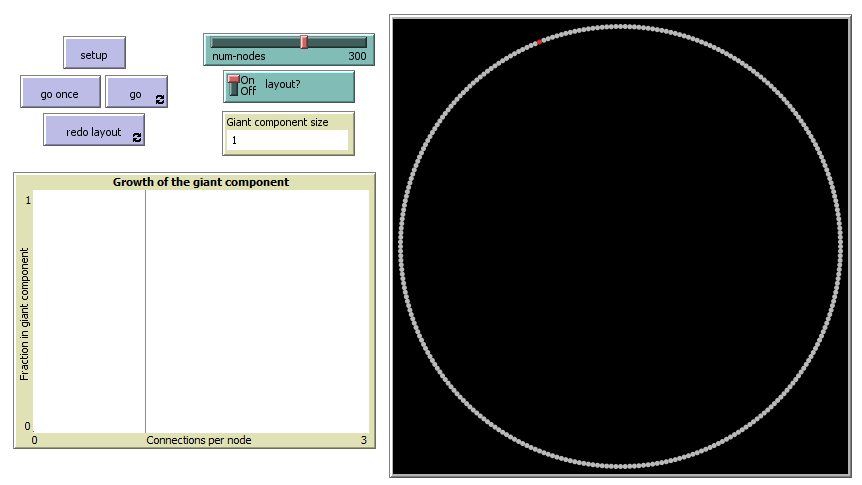
\includegraphics[width=0.7\textwidth]{img/im1}
  \caption{Distribución inicial de la red en NetLogo.}
  \label{im1}
\end{figure}

Si pulsamos el botón \texttt{go}, empieza la simulación y se van añadiendo enlaces de forma aleatoria entre los nodos de la red. En la \hyperref[im2]{Figura \ref{im2}} podemos ver la red cuando el número medio de enlaces que tienen los nodos alcanzan el valor 1 y en la \hyperref[im3]{Figura \ref{im3}} al final de la simulación.

\begin{figure}[H]
    \centering
    \mbox{
        \subfigure[Momento con número medio de enlaces igual a 1.] {
            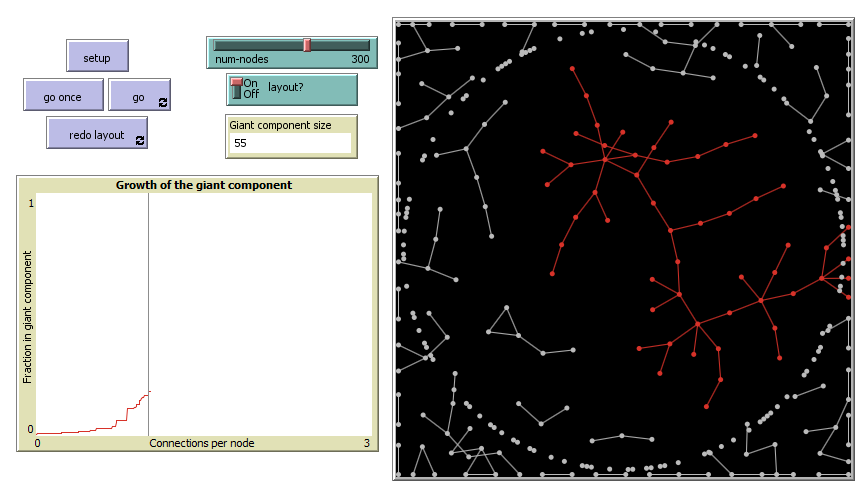
\includegraphics[width=0.5\textwidth]{img/im2}
            \label{im2}
        }
        \qquad
        \subfigure[Final de la simulación.] {
            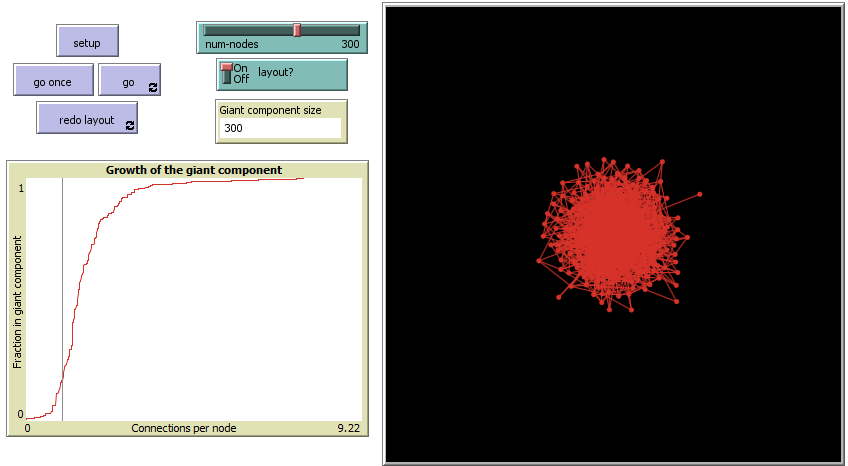
\includegraphics[width=0.5\textwidth]{img/im3}
            \label{im3}
        }
    }
    \caption{Momentos de la simulación}
    \label{im_ej1}
\end{figure}

Al alcanzar el número medio de enlaces igual a 1 (\hyperref[im2]{Figura \ref{im2}}), podemos ver que ya se ha formado una componente conexa de un tamaño considerable, siendo la ``componente gigante'', aunque aún existen un montón de pequeñas islas o componentes conexas de menor tamaño, y muchos más nodos sin ningún enlace. En ella podemos ver cómo la componente gigante corresponde a las características de dicho nombre.

\subsection{Pregunta 2: ¿Qué ocurre cuando la curva del gráfico tiene una pendiente más pronunciada?}

A partir de este momento, la curva que podemos ver en la gráfica en la \hyperref[im3]{Figura \ref{im3}}, podemos ver que crece muchísimo más rápido al ir conectándose entre sí las distintas componentes, generando una componente gigante muchísimo más grande, y haciendo subir mucho el número medio de enlaces que tiene cada nodo, hasta que se consigue una componente gigante que engloba a todos los nodos.

El número de enlaces que tiene cada nodo aumenta tan rápido al pasar el grado medio 1 porque, al ser aleatorio totalmente, es más fácil que se añadan más aristas a la componente gigante que a los nodos aislados. Es por esto por lo que crece tan rápido el grado medio pero tarda ``tanto'' en englobar a todos los nodos.

Esto lo podemos justificar de forma más adecuada haciendo uso de lo siguiente:

Sea $u = 1 - \frac{N_G}{N}$ el número de nodos que no pertenecen a la componente gigante y $N_G$ el número de nodos que están en esta. Para que un nodo $i$ pertenezca a esta componente gigante, debe estar conectado a otro nodo $j$ que sí lo esté. 

Si $i$ no pertenece a la componente gigante, puede ser por lo siguiente:
\begin{enumerate}
  \item El nodo $i$ no está conectado al nodo $j$, lo que tiene una probabilidad de $1-p$.
  \item El nodo $i$ está conectado a $j$, pero ninguno de los dos están conectados a la componente gigante, lo que tiene una probabilidad $p\cdot u$.
\end{enumerate}

Entonces, la probabilidad de que $i$ no esté en la componente gigante por medio de una conexión con un nodo $j$ es igual a $1-p + p \cdot u$, y la probabilidad de que no esté enlazado a la componente gigante por cualquier otro nodo es $(1-p+p\cdot u)^{N-1}$. Por tanto tenemos que $$u = (1-p+p\cdot u)^{N-1}$$

Si tenemos en cuenta que $p=\frac{<k>}{N-1}$ y aplicamos las reglas de los logaritmos, podemos desarrollar esta expresión como sigue a continuación:

\begin{displaymath}
  \ln(u) = \ln\left[\left(1 - \frac{<k>}{N-1} + \frac{<k>}{N-1}\cdot u\right)^{N-1}\right]
\end{displaymath}
\begin{displaymath}
\begin{array}{lcl}
  \ln(u) &=& (N-1)\ln\left[1 - \frac{<k>}{N-1}(1-u)\right] \\
  &\approx &- \cancel{(N-1)} \frac{<k>}{\cancel{N-1}}(1-u) \\
  & = &- <k>(1-u)
\end{array}
\end{displaymath}

Si transformamos esta ecuación logarítmica en una exponencial, obtenemos lo siguiente $$u=e^{- <k>(1-u)}$$

Si $S$ es la fracción de nodos pertenecientes a la componente conexa, tenemos lo siguiente:

\begin{displaymath}
  S = \frac{N_G}{N} \rightarrow S = 1 - u
\end{displaymath}
\begin{displaymath}
  S = 1 - e^-<k>S
\end{displaymath}

Con esto podemos ver cómo el crecimiento del número de nodos y enlaces en la red crece de forma exponencial en función del número de nodos que tenga la componente gigante y del grado medio de la red.

\subsection{Pregunta 3: ¿En qué difiere el gráfico obtenido para un pequeño número de nodos con el obtenido con un gran número de nodos?}

En apartados anteriores hemos visto la gráfica para una red con 300 nodos y el porqué del crecimiento de la gráfica. A continuación, en la \hyperref[im_ej3]{Figura \ref{im_ej3}}, podemos ver la evolución de la gráfica y la red durante la simulación, para una red con 10 nodos.

\begin{figure}[H]
    \centering
    \mbox{
        \subfigure[Momento inicial de la simulación.] {
            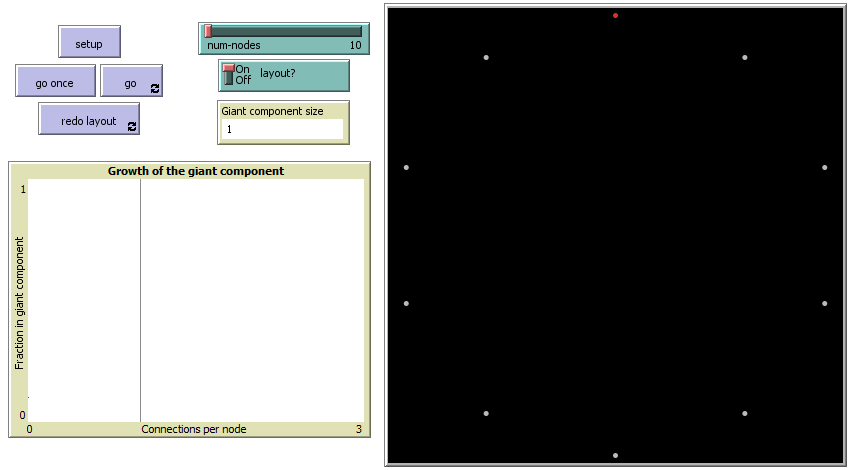
\includegraphics[width=0.5\textwidth]{img/im4}
            \label{im4}
        }
    }
    \mbox{
        \subfigure[Momento con número medio de enlaces igual a 1.] {
            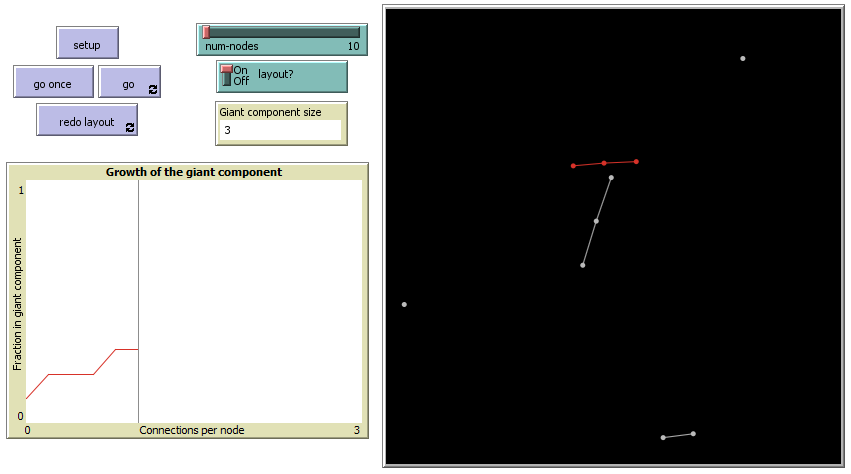
\includegraphics[width=0.5\textwidth]{img/im5}
            \label{im5}
        }
        \qquad
        \subfigure[Final de la simulación.] {
            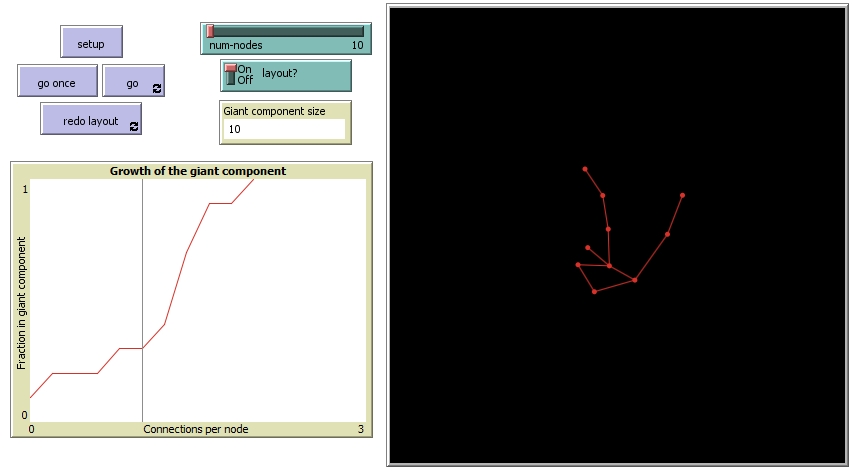
\includegraphics[width=0.5\textwidth]{img/im6}
            \label{im6}
        }
    }
    \caption{Momentos de la simulación para una red pequeña de 10 nodos.}
    \label{im_ej3}
\end{figure}

La única diferencia entre la gráfica que podemos ver en la \hyperref[im3]{Figura \ref{im3}} en la red de 300 nodos con la red de 10 nodos en la \hyperref[im6]{Figura \ref{im6}} es que la gráfica crece antes en la red de menor tamaño, pero el comportamiento es el mismo. Esto se debe a que las ecuaciones $u=e^{- <k>(1-u)},$ $S = 1-e^{-<k>S}$ son generales para las redes aleatorias, y es por eso por lo que se comportan de forma similar, aunque la convergencia más rápida se debe al menor número de nodos.

\subsection{Pregunta 4: ¿Cuánto varía el gráfico de una ejecución a otra?}

Para ver cómo varía el gráfico de una ejecución a otra, he realizado cuatro simulaciones en una red de 200 nodos, viendo cómo varía la gráfica en cada ejecución. En la \hyperref[im_ej4]{Figura \ref{im_ej4}}

\begin{figure}[H]
    \centering
    \mbox{
        \subfigure[Resultado para la primera simulación.] {
            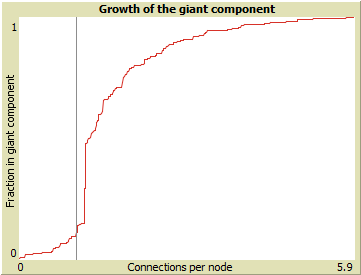
\includegraphics[width=0.5\textwidth]{img/im7}
            \label{im7}
        }

        \subfigure[Resultado para la segunda simulación.] {
            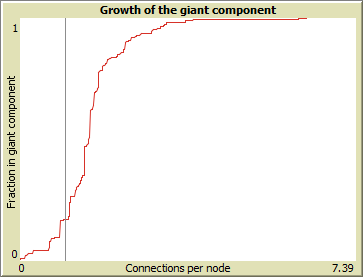
\includegraphics[width=0.5\textwidth]{img/im8}
            \label{im8}
        }
    }
    \mbox{
        \subfigure[Resultado para la tercera simulación.] {
            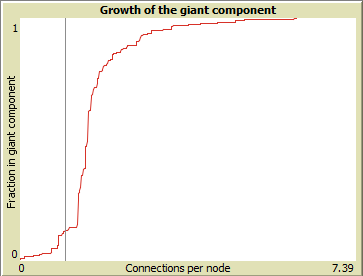
\includegraphics[width=0.5\textwidth]{img/im9}
            \label{im9}
        }
        \subfigure[Resultado para la cuarta simulación.] {
            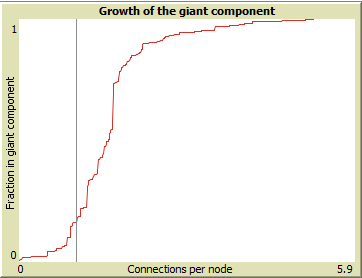
\includegraphics[width=0.5\textwidth]{img/im10}
            \label{im10}
        }
    }
    \caption{Resultados de las gráficas para cada simulación.}
    \label{im_ej4}
\end{figure}

En estas gráficas, podemos ver que la variación del gráfico en cada una de las simulaciones es muy pequeña, presentando todas el mismo comportamiento. las pequeñas variaciones que surgen de una simulación a otra, dependen del componente aleatorio que existe en la simulación, afectando más o menos a la evolución del gráfico, pero todas presentan ese comportamiento exponencial a partir del grado medio igual a 1.

\subsection{Formas de hacer que algunos nodos sean más atractivos para conectarse que otros. ¿Cómo influiría eso en la formación de la componente gigante?}

En las redes anteriores todos tienen la misma probabilidad de conectarse a cualquier otro nodo, por lo que no hay ningún nodo preferente frente a otro. Una forma de cambiar este comportamiento es hacer que los nodos con un mayor grado tengan una mayor probabilidad de que se les conecte otro nodo distinto que los que tienen un grado más pequeño. Es decir, que es más probable conectarse a los hubs que a otros nodos.

En NetLogo, podemos hacer una pequeña simulación con el ejemplo de \textit{Preferential Attachment} que se encarga de realizar una simulación haciendo esto, solo que genera dos nodos con un enlace y luego va generando nuevos nodos que se van conectando a los dos primeros, dando más prefencia a los nodos con mayor grado.

En la \hyperref[im_ej5]{Figura \ref{im_ej5}} podemos ver los resultados de la simulación con NetLogo.

\begin{figure}[H]
    \centering
    \mbox{
        \subfigure[Momento inicial de la simulación.] {
            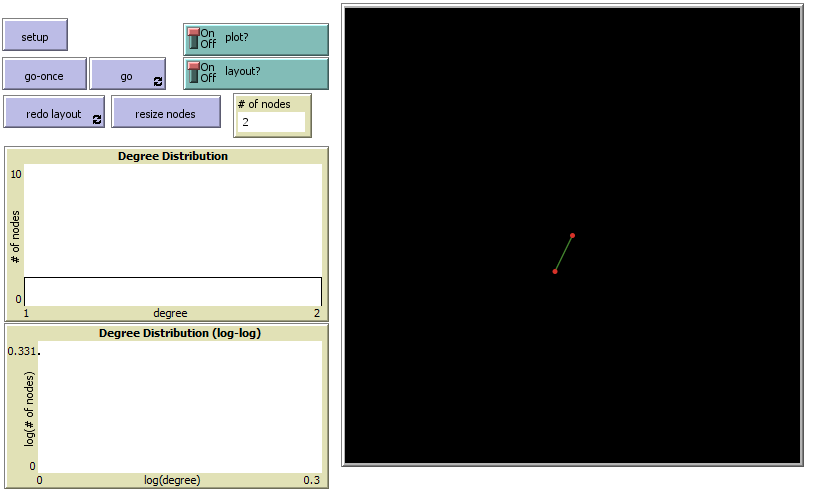
\includegraphics[width=0.5\textwidth]{img/im11}
            \label{im11}
        }
    }
    \mbox{
        \subfigure[Momento a mitad de la simulación.] {
            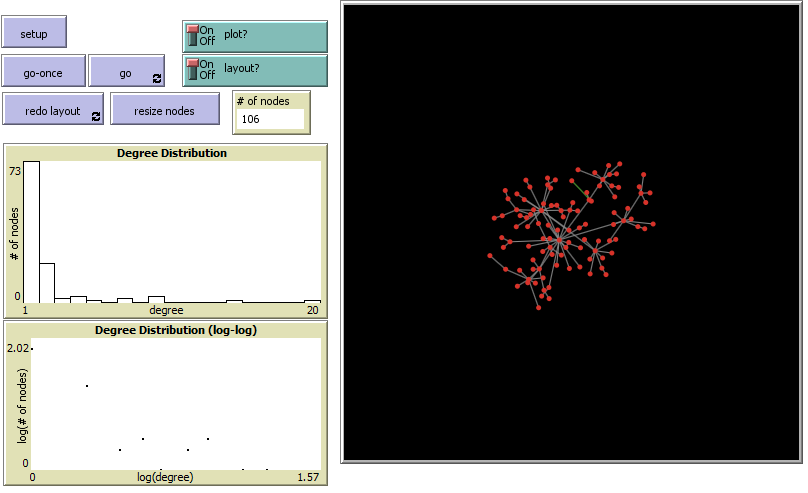
\includegraphics[width=0.5\textwidth]{img/im12}
            \label{im12}
        }
        \qquad
        \subfigure[Final de la simulación.] {
            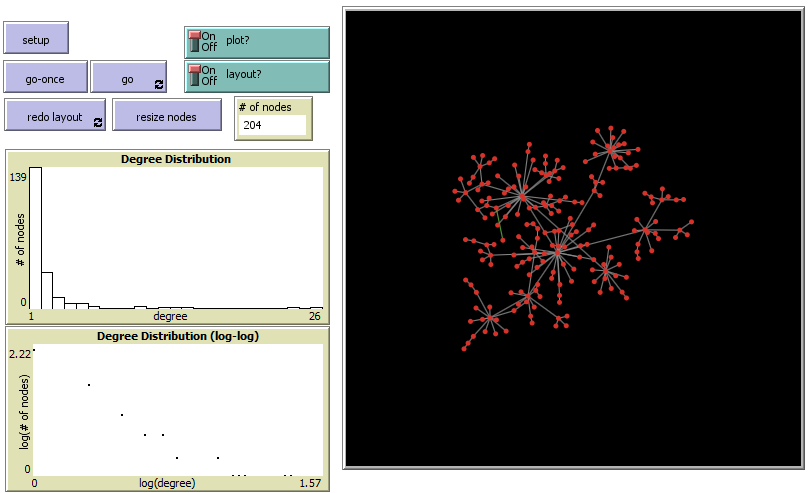
\includegraphics[width=0.5\textwidth]{img/im13}
            \label{im13}
        }
    }
    \caption{Momentos de la simulación con Preferential Attachment.}
    \label{im_ej5}
\end{figure}

En estas imágenes podemos ir viendo la evolución de la red a lo largo del tiempo, y vemos cómo los nodos se van uniendo a los nodos que tienen un mayor grado. Si estos nodos estuvieran sueltos en la red, irían formando componentes conectándose al nodo con mayor grado, generando una componente conexa como la que se ve en la \hyperref[im13]{Figura \ref{im13}}. Pero este comportamiento ya no es el de una red aleatoria, ya que podemos ver en las gráficas que aparecen en cada imagen cómo la distribución de grados y su distribución ultralogarítmica, la red se comporta de forma similar a una red de libre escala.

\section{Dos Componentes Gigantes de una Red Aleatoria}

\subsection{¿Cuánto tiempo se necesita para que las dos componentes gigantes se fusionen?}

En este caso, se ha generado una red con 90 nodos, y los parámetros de layout por defecto que vienen en el modelo. En la \hyperref[imej2]{Figura \ref{imej2}} podemos ver la configuración inicial de nodos, y las dos componentes gigantes separadas.

\begin{figure}[H]
    \centering
    \mbox{
        \subfigure[Configuración inicial de la simulación.] {
            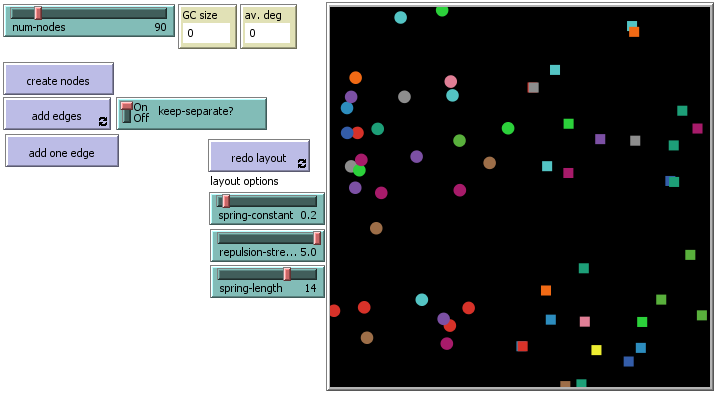
\includegraphics[width=0.5\textwidth]{img/im14}
            \label{im14}
        }
        \qquad
        \subfigure[Dos componentes gigantes separadas] {
            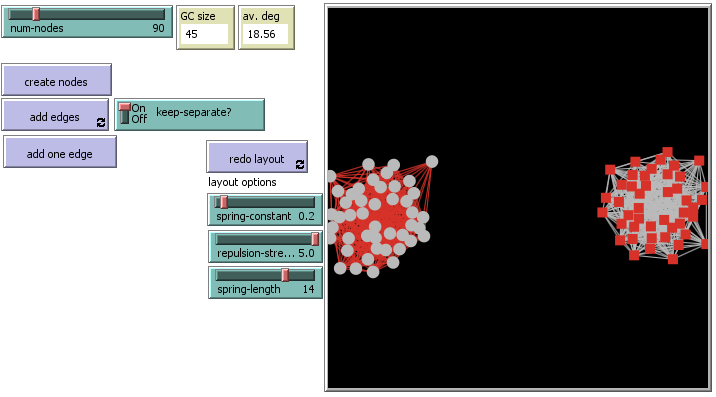
\includegraphics[width=0.5\textwidth]{img/im15}
            \label{im15}
        }
    }
    \caption{Pasos previos para la simulación.}
    \label{imej2}
\end{figure}

Una vez aquí, tenemos bien diferenciadas ambas comunidades, repartidas en dos componentes gigantes para cada tipo de nodo. A partir de aquí, empezaremos a contar el número de \textit{ticks} o pasos necesarios hasta que las dos componentes queden mezcladas.

Lo más sencillo y cómodo para hacer esto es añadir en el código del modelo \texttt{reset-ticks} en la función \texttt{create-turtles} para resetear el número de ticks al presionar el botón \textit{create nodes}, y añadir en la función \texttt{add-edge} la orden \texttt{tick}, para incrementar el contador de ticks cada vez que se añade una arista. De esta forma, podemos hacer la simulación mucho más rápida y cómodamente que ir contando los clicks que hacemos con el ratón a mano. A continuación, en \hyperref[imej23]{Figura \ref{imej23}}, podemos ver la evolución de la red y el número de pasos necesarios.

\begin{figure}[H]
    \centering
    \mbox{
      \subfigure[Estado de la red tras 2 \textit{ticks}.]{
        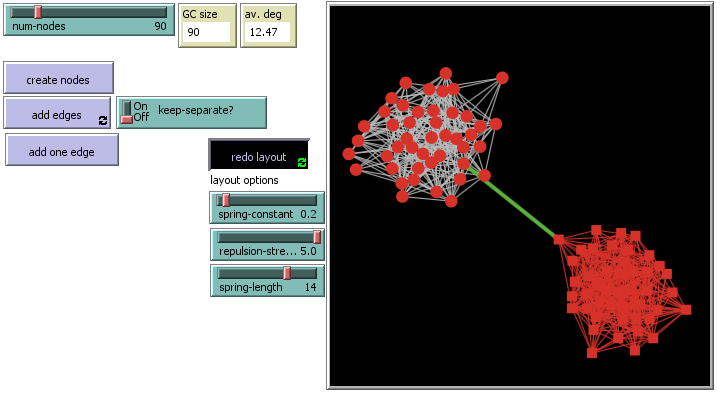
\includegraphics[width=0.5\textwidth]{img/im23}
        \label{im23}
      }
    }
    \mbox{
        \subfigure[Estado de la red tras 11 \textit{ticks}.] {
            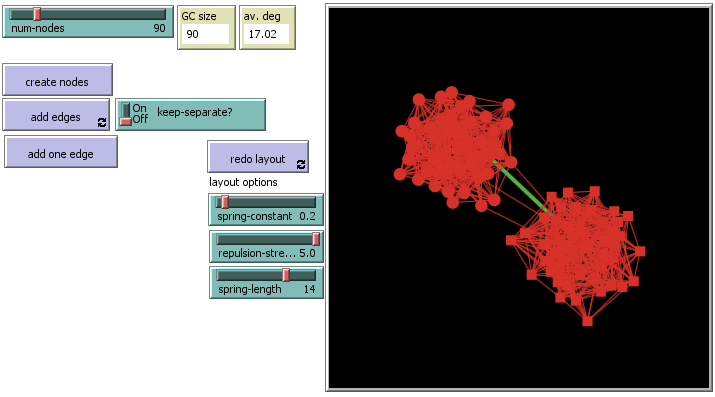
\includegraphics[width=0.5\textwidth]{img/im16}
            \label{im16}
        }
        \qquad
        \subfigure[Estado de la red tras 100 \textit{ticks}.] {
            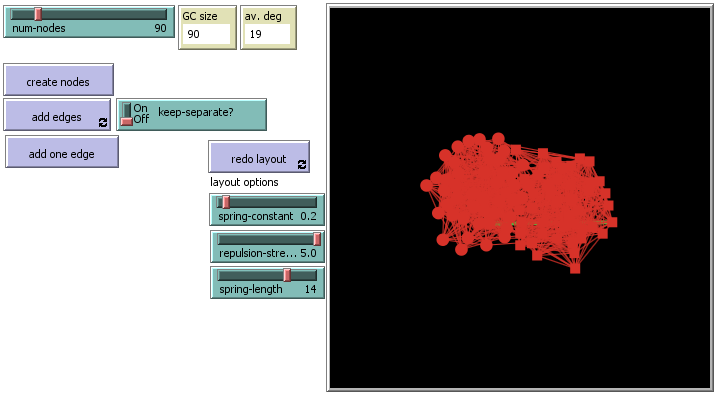
\includegraphics[width=0.5\textwidth]{img/im17}
            \label{im17}
        }
    }
    \caption{Pasos previos para la simulación.}
    \label{imej23}
\end{figure}

En este estado, con añadir dos enlaces (\hyperref[im23]{Figura \ref{im23}}), ya las dos componentes gigantes pasan a ser una sola componente conexa. En la \hyperref[im16]{Figura \ref{im16}} podemos ver como en tan solo 11 pasos, la red ya forma una sola componente conexa y ambas componentes se empiezan a mezclar, mientras que en la \hyperref[im17]{Figura \ref{im17}} ambas componentes ya están muy fusionadas, en tan solo 100 pasos, formando una componente gigante altamente densa, con grado medio igual a 19.

Esto se debe a que ambas componentes tienen un alto grado medio, y en cuanto se establece un enlace entre ambas componentes, si seguimos las ecuaciones $u=e^{- <k>(1-u)},$ $S = 1-e^{-<k>S}$, son altamente dependientes del grado medio de la red, y al ser tan alto en este caso, su comportamiento exponencial es muy fuerte, por lo que en pocos pasos, ambas componentes estarán fuertemente fusionadas, tal y como hemos podido comprobar.

\subsection{¿Tiene sentido que los grafos aleatorios sólo generen una componente gigante?}

Sí, ya que como todos los nodos pueden conectarse con todos y todos tienen la misma probabilidad de conectarse, tiene sentido que sólo se genere una componente gigante como se ha podido comprobar en el caso anterior al cabo de muchas iteraciones.

\section{Componente Gigante de un Retículo 2D}

\subsection{¿Existe un valor crítico de $p$ a partir del cual se forma una componente gigante?}

Para analizar el valor crítico de $p$, he realizado una ejecución completa que va variando el valor de $p$ desde 0 hasta 0.9. Con esto, se puede obtener la gráfica de la \hyperref[im18]{Figura \ref{im18}}, donde podemos ver la variación en el tamaño de la componenente gigante según el valor de $p$.

\begin{figure}[H]
  \centering
  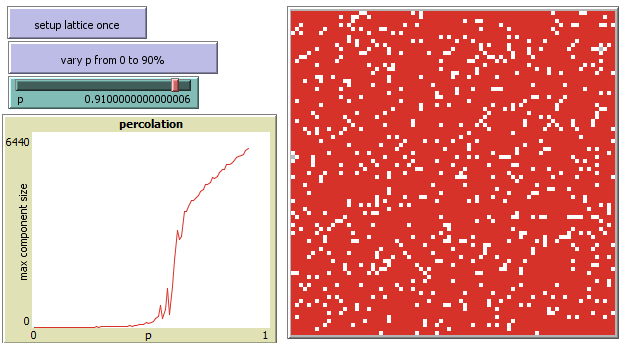
\includegraphics[width=0.7\textwidth]{img/im18}
  \caption{Gráfica de distribución del tamaño de la componente gigante según el valor de $p$.}
  \label{im18}
\end{figure}

En esta imagen podemos ver cómo el tamaño de la componente gigante se mantiene más o menos constante, casi de forma asintótica en 0, siendo el máximo en 6440. Pero en $p=0.5$ el tamaño de la componente gigante empieza a crecer de forma casi exponencial, muy bruscamente, suavizándose ese crecimiento con un valor de $p \approx 0.61$. Es por esto, por lo que nos vamos a analizar en los valores cercanos a 0.5 el comportamiento de la simulación y para ello, podemos ver la \hyperref[imej24]{Figura \ref{imej24}}:

\begin{figure}[H]
    \centering
    \mbox{
        \subfigure[Componente gigante con $p = 0.52$.] {
            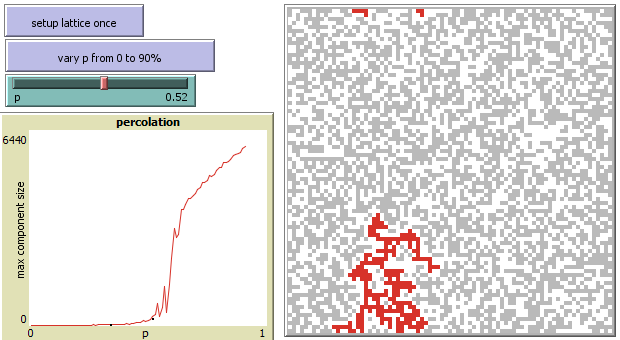
\includegraphics[width=0.5\textwidth]{img/im19}
            \label{im19}
        }
        \qquad
        \subfigure[Componente gigante con $p = 0.53$.] {
            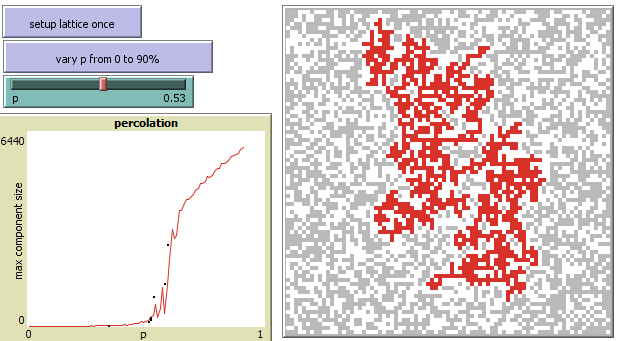
\includegraphics[width=0.5\textwidth]{img/im20}
            \label{im20}
        }
    }
    \mbox{
        \subfigure[Componente gigante con $p = 0.58$.] {
            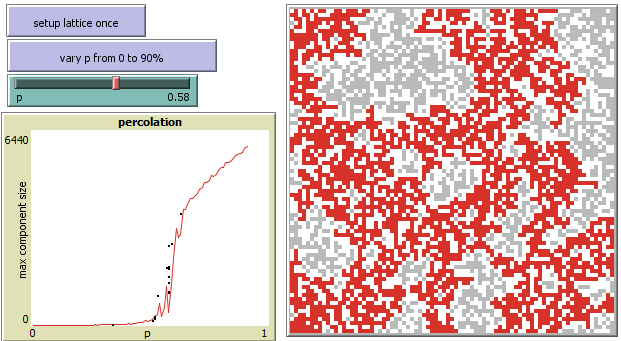
\includegraphics[width=0.5\textwidth]{img/im21}
            \label{im21}
        }
        \qquad
        \subfigure[Componente gigante con $p = 0.63$.] {
            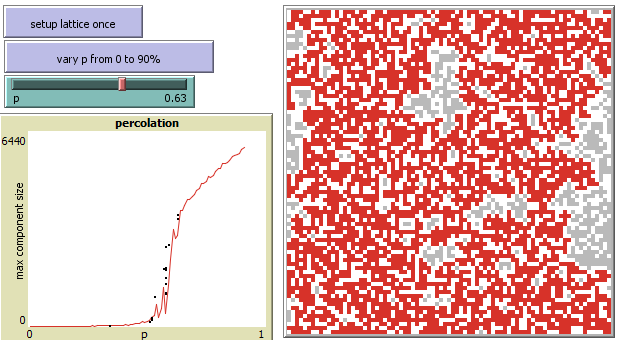
\includegraphics[width=0.5\textwidth]{img/im22}
            \label{im22}
        }
    }
    \caption{Pasos previos para la simulación.}
    \label{imej24}
\end{figure}

En \hyperref[im19]{Figura \ref{im19}} podemos ver como con $p=0.52$, la componente gigante que se consigue representa un pequeño porcentaje de la red, mientras que si aumentamos este valor una centésima más, la componente gigante aumenta muchísimo su tamaño, como se puede ver en \hyperref[im20]{Figura \ref{im20}}.

Mientras tanto, en las imágenes de las \hyperref[im21]{Figura \ref{im21}} y \hyperref[im22]{Figura \ref{im22}}, podemos ver cómo para los valores de $p = 0.58$ y $p=0.63$, las componentes gigantes obtenidas son muchísimo más grandes.

Por esto, podemos ver que el valor crítico de $p$ a partir del cual se forma una componente gigante es $p\approx0.55$, con un pequeño porcentaje de error debido al componente aleatorio de la red. Una vez que $p$ sobrepase este valor, es más probable que los nodos estén altamente conexos, por lo que a mayor probabilidad, mayor será la componente conexa de la red.

\end{document}
